% V2 working paper: compact ICAPS-style presentation of the Playbook model.
\documentclass[letterpaper]{article}
\usepackage[draft]{aaai2026}
\usepackage{times}
\usepackage{helvet}
\usepackage{courier}
\usepackage[hyphens]{url}
\usepackage{graphicx}
\urlstyle{rm}
\def\UrlFont{\rm}
\usepackage[numbers,square]{natbib}
\usepackage{caption}
\frenchspacing
\setlength{\pdfpagewidth}{8.5in}
\setlength{\pdfpageheight}{11in}

\usepackage{amsthm}

\theoremstyle{definition}
\newtheorem{definition}{Definition}

\usepackage{amsmath,amssymb}
\usepackage{algorithm}
\usepackage{algorithmic}
\usepackage{newfloat}
\usepackage{listings}
\usepackage{tikz}
\usetikzlibrary{arrows.meta,positioning,calc}

\DeclareCaptionStyle{ruled}{labelfont=normalfont,labelsep=colon,strut=off}
\lstset{
  basicstyle=\footnotesize\ttfamily,
  numbers=none,
  aboveskip=3pt,
  belowskip=3pt,
  showstringspaces=false,
  tabsize=2,
  breaklines=true
}
\floatstyle{ruled}
\newfloat{listing}{tb}{lst}{}
\floatname{listing}{Listing}

\pdfinfo{
/TemplateVersion (2026.1)
}
\setcounter{secnumdepth}{1}

\title{Finite Agent Machines}
\author{Dustin Dannenhauer}
\affiliations{
  Delegance AI\\
  \texttt{dustin@delegance.ai}
}

\begin{document}
\maketitle

% ---------------------------------------------------------------------------
% Fresh draft: replace each TBD as you rewrite the paper.
% ---------------------------------------------------------------------------
\begin{abstract}
TBD
\end{abstract}

\section{Introduction}

Giving an AI an open-ended goal to run with creates a fundamental problem of trust: the same system decides what is worth pursuing and what will count as success. In exploratory work, we do not yet know what we will find or which findings will matter. An investigation of an unfamiliar software system, for example, may begin with the aim of identifying worthwhile improvements, while leaving the relevant problems and possible solutions to be discovered. Evidence gathered during the investigation helps determine what to pursue and what would count as a useful result. A concrete end state and a complete criterion for success may therefore be unavailable before the work begins. Even when the desired outcome is known, verifying that the outcome has been achieved may be costly or inconclusive.

Exploratory work can be understood as a search whose concrete objectives emerge and change as evidence accumulates. We introduce \emph{nondeterministic finite agent machines} (FAMs)\footnote{Intentionally echoes finite state machines}, a model for process-driven agentic teams that makes the search process explicit and interpretable by defining how agents investigate possibilities, assess findings, and decide what to pursue next. FAMs ensure that work proceeds in a permitted order and make the path to a result inspectable. Confidence in the result can then draw on the reliability of the search process and evidence that it was followed, even when the result itself could not be specified in advance or conclusively verified.

The same FAM can therefore produce different executions. An agentic transition may divide a problem into several investigations or produce findings that enable different continuations, while the available types of investigation and continuation remain defined by the FAM. A FAM defines a finite repertoire of predefined agentic transitions, each admitting multiple possible outcomes. Agents determine how those transitions are applied to the work at hand, allowing the search to develop through discoveries without requiring its concrete branches to be enumerated in advance.

Here, \emph{finite} refers to the set of authored transition schemas. Finite transition schemas do not imply finitely many artifact states: executions can accumulate new artifact files that affect subsequent work. The number of concrete branches and iterations need not be fixed in advance.

Recent projects such as Compound Engineering \citep{everyCompoundEngineering}, Compound Writing \citep{everyCompoundWriting}, and Research--Plan--Implement (RPI) \citep{dex2025context} organize agent work through reusable skills and staged procedures. These approaches make a process explicit, but procedural instructions expressed in prompts do not by themselves guarantee adherence. Where a coordinating agent selects activities, judges whether their requirements have been met, and decides what happens next, the process remains dependent on that agent's interpretation. An agent may omit a prerequisite, advance on insufficient evidence, or allow an unsupported assumption to shape subsequent work. FAMs address this coordination problem by making declared dependencies conditions for execution, so that following the prescribed process does not rely solely on the coordinating agent's willingness or ability to follow instructions.

We implement this model in Alinery\footnote{\url{https://github.com/deleganceai/alinery}}, where a Playbook specifies a particular FAM and the Playbook engine executes it. A single Playbook can produce many different executions, each developing according to the evidence generated during the work. The remainder of this paper develops the FAM model and its execution semantics, relates it to existing approaches, and describes its implementation in Alinery.

% New implementation-aligned section. Existing manuscript retained below.
% Source baseline: Alinery 91213afb6e39b821cbf4bf5aed3df813cb2f46b7.
\section{Finite Agent Machines}
\label{sec:fam-definition-execution}








A Finite Agent Machine (FAM) defines an abstract state space, a finite set of
agentic operations, and rules governing when those operations may run. An
execution engine enforces these rules, providing hard guardrails on how the
agents' work is coordinated. A state is a set of available artifact filenames;
agents interpret and create the files' contents. An
execution engine binds
operations to available inputs, records the resulting executions, and
enforces the conditions for passing their outputs to other agents. A single
definition can therefore generate different numbers of executions and
different chains of evidence without changing its authored operations.

\begin{definition}[Finite Agent Machine]
A FAM is a transition system
\[
  \mathcal{F}=(\mathcal{A},\mathcal{S},s_0,\rightarrow),
\]
where $\mathcal{A}$ is a finite set of authored agent operation schemas,
$\mathcal{S}$ is a set of artifact states, $s_0\in\mathcal{S}$ is the
initial state, and
$\rightarrow\;\subseteq\;\mathcal{S}\times\mathcal{A}\times\mathcal{S}$
is the transition relation. Each state is a finite set of available artifact
filenames. A transition \mbox{$s\xrightarrow{\alpha}s'$} represents a completed
invocation of operation $\alpha$ using artifacts named in $s$ and publishing
output artifacts whose filenames form a set $P$, so that $s'=s\cup P$.
\end{definition}

Here, \emph{finite} refers to the authored operation set $\mathcal{A}$.
The same operation may publish different sets of artifact filenames from
the same state, giving rise to more than one possible successor. Repeated invocations
can add new filenames, so the number of reachable states may be unbounded
and an execution need not terminate.

% New formalism outline; draft each subsection separately.
\subsection{Artifacts and States}

An \emph{artifact} is a file that carries information used or produced by
an agent operation, such as a task description, source assessment, or
proposed solution. Let $\mathcal{D}$ denote the universe of artifact filenames.
Each state $s\in\mathcal{S}$ is a finite subset of $\mathcal{D}$.
The initial state $s_0$ contains the filenames of the initial input artifacts.

Artifacts with different filenames remain distinct even when they serve the
same purpose or contain identical text. Reading an artifact does not remove
its filename from the state, so the same artifact can support several later
operations.

\subsection{Agent Operations}

An \emph{agent operation schema} $\alpha\in\mathcal{A}$ is a reusable
specification of work for an agent. We write
\[
  \alpha=(I_\alpha,O_\alpha,\xi_\alpha).
\]
The input and output specifications are families of permitted filename sets,
\[
  I_\alpha,\ O_\alpha\subseteq\mathcal{P}_{\mathrm{fin}}(\mathcal{D}),
\]
where $\mathcal{P}_{\mathrm{fin}}(\mathcal{D})$ denotes the finite subsets of
$\mathcal{D}$. The execution specification $\xi_\alpha$ supplies the agent's
instructions and execution configuration.

An \emph{invocation} is one execution of a schema. Its input filenames must
form a set in $I_\alpha$ and all be present in the current state. The agent
interprets the corresponding files under the specified instructions, and
its published output filenames must form a set in $O_\alpha$. Neither
specification predetermines file contents. The same schema, $\alpha$, can be invoked
repeatedly with different inputs, so additional executions do not enlarge
the authored operation set $\mathcal{A}$.

\subsection{Agentic Transitions}

For a completed invocation of schema $\alpha$ from state $s$, let $B$ be
its set of input filenames and $P$ its set of published output filenames.
The invocation must satisfy
\[
  B\in I_\alpha,\qquad B\subseteq s,\qquad P\in O_\alpha,\qquad P\ne\varnothing,
\]
and produces the \emph{agentic transition}
\[
  s\xrightarrow{\alpha}s',\qquad s'=s\cup P.
\]
All filenames in $s$ remain available in $s'$.

Each invocation publishes one or more artifacts, whose filenames form $P$.
By choosing which permitted outputs to publish, the agent can satisfy the
input requirements of different subsequent operations, enabling conditional
branching. Published artifacts can support several continuations, while
fresh artifacts that supply inputs to an earlier operation can enable
another iteration.

\subsection{Executions}

A \emph{rollout}, or execution of a FAM, is a finite or infinite sequence of
transitions beginning at the initial state $s_0$:
\[
  s_0\xrightarrow{\alpha_1}s_1
  \xrightarrow{\alpha_2}s_2
  \xrightarrow{\alpha_3}\cdots,
\]
where each $\alpha_i\in\mathcal{A}$ and each transition belongs to the
relation $\rightarrow$.

The same schema may appear repeatedly in a rollout, and different rollouts
of the same FAM may follow different sequences of transitions. Repeating
an operation can extend the accumulated state with new artifact filenames.

\section{Motivating Examples}
\label{sec:fam-literature-example}

To illustrate how a FAM organizes agent work, consider a team conducting a
literature review. Given a research question, the agents find relevant papers,
assess their findings, and synthesize a report.
Figure~\ref{fig:fam-literature-variants} shows three FAM definitions:
one that branches across papers, one that loops as new sources are discovered,
and one that combines both structures.

% Requires tikz with arrows.meta; designed for a 17.8 cm two-column text width.
% Deliberately unscaled: operation labels are 8.5 pt and annotations are 8 pt.
\begin{figure*}[t]
\centering
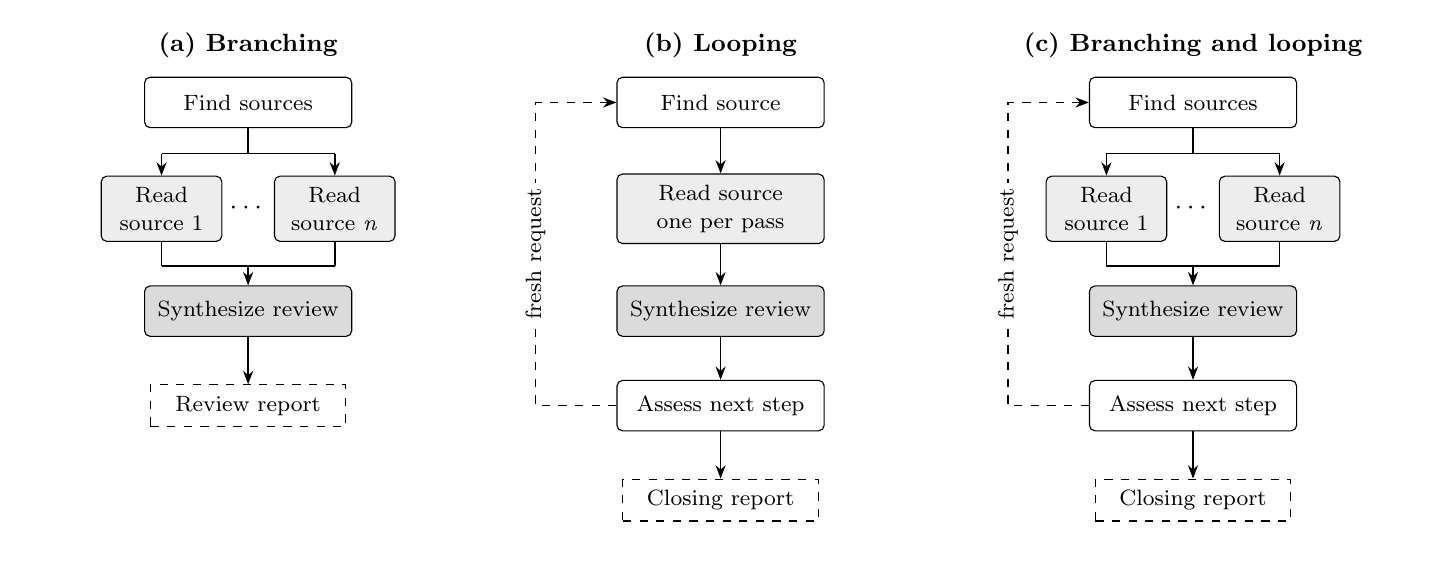
\begin{tikzpicture}[
  operation/.style={draw,rounded corners=2pt,align=center,
    text width=2.35cm,minimum height=.64cm,inner sep=4pt,
    font=\fontsize{8.5}{10}\selectfont},
  reader/.style={operation,fill=black!7},
  synthesis/.style={operation,fill=black!14},
  artifact/.style={draw,dashed,align=center,text width=2.2cm,
    minimum height=.53cm,inner sep=4pt,
    font=\fontsize{8.5}{10}\selectfont},
  handoff/.style={-{Stealth[length=1.7mm]},semithick},
  recurrence/.style={handoff,dashed},
  panel/.style={align=center,text width=5.5cm,inner sep=0pt,
    font=\fontsize{9.5}{11}\selectfont\bfseries},
  annotation/.style={align=center,font=\fontsize{8}{9}\selectfont},
  request/.style={annotation,rotate=90,fill=white,inner sep=2pt}
]
% Explicit bounds make the fragment fit without shrinking its text.
\useasboundingbox (-2.8,-5.48) rectangle (14.97,.95);

\begin{scope}
  \node[panel] at (0,.73) {(a) Branching};
  \node[operation] (a-find) at (0,0) {Find sources};
  \node[reader,text width=1.25cm] (a-read-1) at (-1.1,-1.35) {Read\\source 1};
  \node[reader,text width=1.25cm] (a-read-n) at (1.1,-1.35) {Read\\source \textit{n}};
  \node[font=\normalsize] at (0,-1.35) {$\cdots$};
  \node[synthesis] (a-synth) at (0,-2.65) {Synthesize review};
  \node[artifact] (a-report) at (0,-3.85) {Review report};

  \draw[semithick] (a-find.south) -- (0,-.65);
  \draw[semithick] (-1.1,-.65) -- (1.1,-.65);
  \draw[handoff] (-1.1,-.65) -- (a-read-1.north);
  \draw[handoff] (1.1,-.65) -- (a-read-n.north);
  \draw[semithick] (a-read-1.south) -- (-1.1,-2.08);
  \draw[semithick] (a-read-n.south) -- (1.1,-2.08);
  \draw[semithick] (-1.1,-2.08) -- (1.1,-2.08);
  \draw[handoff] (0,-2.08) -- (a-synth.north);
  \draw[handoff] (a-synth) -- (a-report);
\end{scope}

\begin{scope}[xshift=6cm]
  \node[panel] at (0,.73) {(b) Looping};
  \node[operation] (b-find) at (0,0) {Find source};
  \node[reader] (b-read) at (0,-1.35)
    {Read source\\{\fontsize{8}{9}\selectfont one per pass}};
  \node[synthesis] (b-synth) at (0,-2.65) {Synthesize review};
  \node[operation] (b-assess) at (0,-3.85) {Assess next step};
  \node[artifact] (b-report) at (0,-5.05) {Closing report};

  \draw[handoff] (b-find) -- (b-read);
  \draw[handoff] (b-read) -- (b-synth);
  \draw[handoff] (b-synth) -- (b-assess);
  \draw[handoff] (b-assess) -- (b-report);
  \draw[recurrence] (b-assess.west) -- (-2.35,-3.85)
    -- node[request] {fresh request} (-2.35,0) -- (b-find.west);
\end{scope}

\begin{scope}[xshift=12cm]
  \node[panel] at (0,.73) {(c) Branching and looping};
  \node[operation] (c-find) at (0,0) {Find sources};
  \node[reader,text width=1.25cm] (c-read-1) at (-1.1,-1.35) {Read\\source 1};
  \node[reader,text width=1.25cm] (c-read-n) at (1.1,-1.35) {Read\\source \textit{n}};
  \node[font=\normalsize] at (0,-1.35) {$\cdots$};
  \node[synthesis] (c-synth) at (0,-2.65) {Synthesize review};
  \node[operation] (c-assess) at (0,-3.85) {Assess next step};
  \node[artifact] (c-report) at (0,-5.05) {Closing report};

  \draw[semithick] (c-find.south) -- (0,-.65);
  \draw[semithick] (-1.1,-.65) -- (1.1,-.65);
  \draw[handoff] (-1.1,-.65) -- (c-read-1.north);
  \draw[handoff] (1.1,-.65) -- (c-read-n.north);
  \draw[semithick] (c-read-1.south) -- (-1.1,-2.08);
  \draw[semithick] (c-read-n.south) -- (1.1,-2.08);
  \draw[semithick] (-1.1,-2.08) -- (1.1,-2.08);
  \draw[handoff] (0,-2.08) -- (c-synth.north);
  \draw[handoff] (c-synth) -- (c-assess);
  \draw[handoff] (c-assess) -- (c-report);
  \draw[recurrence] (c-assess.west) -- (-2.35,-3.85)
    -- node[request] {fresh request} (-2.35,0) -- (c-find.west);
\end{scope}
\end{tikzpicture}
\caption{Session patterns specified by three literature-review FAMs. Each
rounded box represents an agent session invoking the named operation. In
(a) and (c), there is one reading session per selected source; the ellipsis
leaves the source count unspecified. These sessions invoke the same
\emph{Read source} schema. Solid arrows show principal artifact dependencies.
Dashed return arrows indicate new passes enabled by fresh requests; dashed
rectangles are output artifacts.}
\label{fig:fam-literature-variants}
\end{figure*}

% Full-page companion to the three literature-review operation patterns.
% Requires tikz with arrows.meta. No scaling: labels are 9--11 pt.
\begin{figure*}[p]
\centering
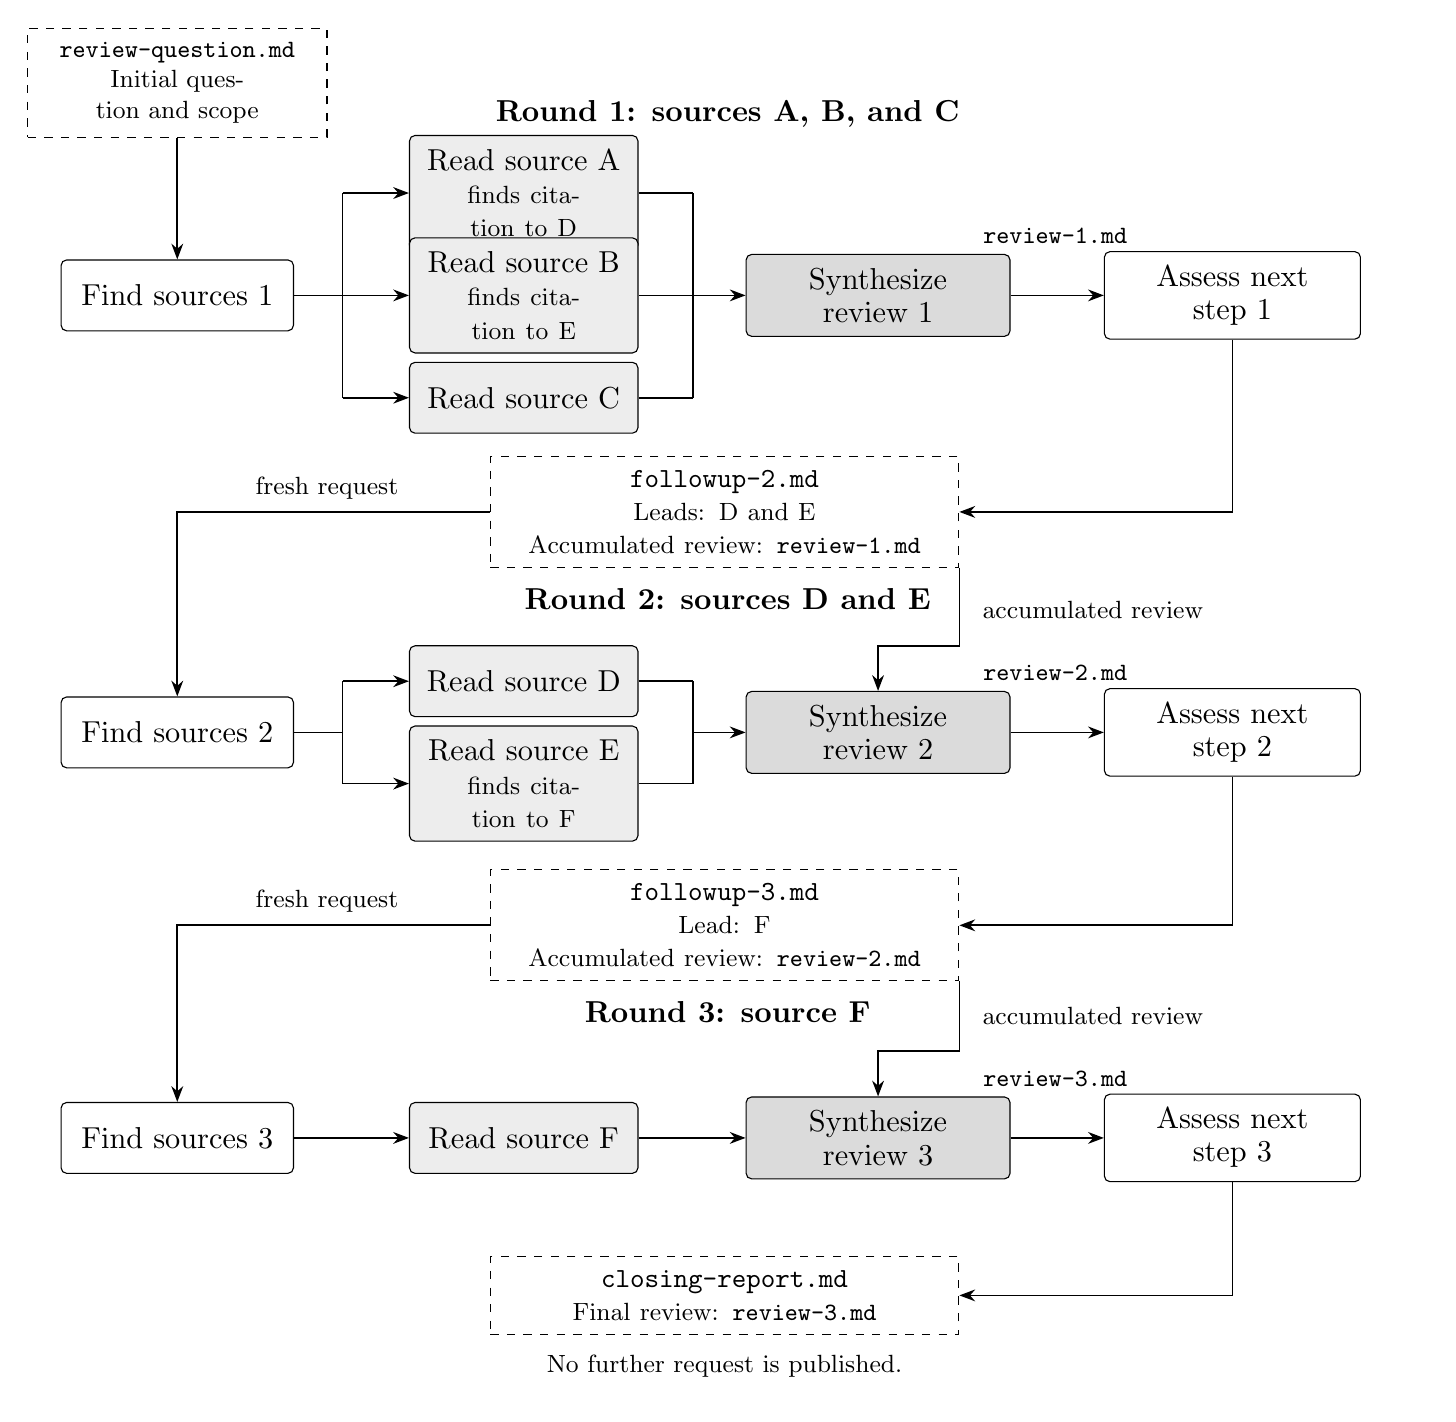
\begin{tikzpicture}[
  execution/.style={draw,rounded corners=2pt,align=center,
    text width=2.6cm,minimum height=.9cm,inner sep=5pt,
    font=\fontsize{10.5}{12}\selectfont},
  reader/.style={execution,fill=black!7,text width=2.55cm},
  synthesis/.style={execution,fill=black!14,text width=3cm},
  assessment/.style={execution,text width=2.9cm},
  artifact/.style={draw,dashed,align=center,text width=5.6cm,
    minimum height=.95cm,inner sep=5pt,
    font=\fontsize{10}{12}\selectfont},
  handoff/.style={-{Stealth[length=2mm]},semithick},
  connector/.style={semithick},
  roundtitle/.style={font=\fontsize{11}{13}\selectfont\bfseries,
    align=center,inner sep=0pt},
  annotation/.style={font=\fontsize{9}{11}\selectfont,
    align=center,fill=white,inner sep=2pt}
]
\useasboundingbox (0,-16.65) rectangle (17.78,.7);

% Initial artifact and the first six completed invocations.
\node[artifact,text width=3.45cm,font=\fontsize{9}{11}\selectfont]
  (question) at (1.9,0)
  {\texttt{review-question.md}\\
   {\fontsize{9}{11}\selectfont Initial question and scope}};
\node[roundtitle] at (8.89,-.4) {Round 1: sources A, B, and C};
\node[execution] (find1) at (1.9,-2.7) {Find sources 1};
\node[reader] (readA) at (6.3,-1.4)
  {Read source A\\{\fontsize{9}{11}\selectfont finds citation to D}};
\node[reader] (readB) at (6.3,-2.7)
  {Read source B\\{\fontsize{9}{11}\selectfont finds citation to E}};
\node[reader] (readC) at (6.3,-4.0) {Read source C};
\node[synthesis] (synth1) at (10.8,-2.7) {Synthesize review 1};
\node[assessment] (assess1) at (15.3,-2.7) {Assess next step 1};
\node[artifact] (followup2) at (8.85,-5.45)
  {\texttt{followup-2.md}\\
   {\fontsize{9}{11}\selectfont Leads: D and E}\\
   {\fontsize{9}{11}\selectfont Accumulated review: \texttt{review-1.md}}};

\draw[handoff] (question) -- (find1);
\draw[connector] (find1.east) -- (4,-2.7);
\draw[connector] (4,-1.4) -- (4,-4.0);
\foreach \source in {A,B,C}{
  \draw[handoff] (4,-2.7 |- read\source.west) -- (read\source.west);
  \draw[connector] (read\source.east) -- (8.45,-2.7 |- read\source.east);
}
\draw[connector] (8.45,-1.4) -- (8.45,-4.0);
\draw[handoff] (8.45,-2.7) -- (synth1.west);
\draw[handoff] (synth1) -- (assess1);
\node[annotation] at (13.05,-1.95) {\texttt{review-1.md}};
\draw[handoff] (assess1.south) -- (15.3,-5.45) -- (followup2.east);

% Five more completed invocations use the same four schemas.
\node[roundtitle] at (8.89,-6.55) {Round 2: sources D and E};
\node[execution] (find2) at (1.9,-8.25) {Find sources 2};
\node[reader] (readD) at (6.3,-7.6) {Read source D};
\node[reader] (readE) at (6.3,-8.9)
  {Read source E\\{\fontsize{9}{11}\selectfont finds citation to F}};
\node[synthesis] (synth2) at (10.8,-8.25) {Synthesize review 2};
\node[assessment] (assess2) at (15.3,-8.25) {Assess next step 2};
\node[artifact] (followup3) at (8.85,-10.7)
  {\texttt{followup-3.md}\\
   {\fontsize{9}{11}\selectfont Lead: F}\\
   {\fontsize{9}{11}\selectfont Accumulated review: \texttt{review-2.md}}};

% The fresh request reaches both source discovery and the next synthesis.
\draw[handoff] (followup2.west) -- (1.9,-5.45) -- (find2.north);
\node[annotation] at (3.8,-5.15) {fresh request};
\draw[handoff] (followup2.south east) |- (10.8,-7.15) -- (synth2.north);
\node[annotation,anchor=west] at (12.05,-6.7) {accumulated review};

\draw[connector] (find2.east) -- (4,-8.25);
\draw[connector] (4,-7.6) -- (4,-8.9);
\foreach \source in {D,E}{
  \draw[handoff] (4,-8.25 |- read\source.west) -- (read\source.west);
  \draw[connector] (read\source.east) -- (8.45,-8.25 |- read\source.east);
}
\draw[connector] (8.45,-7.6) -- (8.45,-8.9);
\draw[handoff] (8.45,-8.25) -- (synth2.west);
\draw[handoff] (synth2) -- (assess2);
\node[annotation] at (13.05,-7.5) {\texttt{review-2.md}};
\draw[handoff] (assess2.south) -- (15.3,-10.7) -- (followup3.east);

% Four final invocations; publication ends without another request.
\node[roundtitle] at (8.89,-11.8) {Round 3: source F};
\node[execution] (find3) at (1.9,-13.4) {Find sources 3};
\node[reader] (readF) at (6.3,-13.4) {Read source F};
\node[synthesis] (synth3) at (10.8,-13.4) {Synthesize review 3};
\node[assessment] (assess3) at (15.3,-13.4) {Assess next step 3};
\node[artifact] (closing) at (8.85,-15.4)
  {\texttt{closing-report.md}\\
   {\fontsize{9}{11}\selectfont Final review: \texttt{review-3.md}}};

\draw[handoff] (followup3.west) -- (1.9,-10.7) -- (find3.north);
\node[annotation] at (3.8,-10.4) {fresh request};
\draw[handoff] (followup3.south east) |- (10.8,-12.3) -- (synth3.north);
\node[annotation,anchor=west] at (12.05,-11.85) {accumulated review};

\draw[handoff] (find3) -- (readF);
\draw[handoff] (readF) -- (synth3);
\draw[handoff] (synth3) -- (assess3);
\node[annotation] at (13.05,-12.65) {\texttt{review-3.md}};
\draw[handoff] (assess3.south) -- (15.3,-15.4) -- (closing.east);
\node[annotation] at (8.85,-16.3) {No further request is published.};
\end{tikzpicture}
\caption{One possible rollout of the branching and looping FAM in
Figure~\ref{fig:fam-literature-variants}(c). Four authored operation schemas
produce 15 completed invocations across three rounds. Each rounded box is
one invocation; dashed boxes identify artifacts. Reading connections
represent the \texttt{request-X.md} and \texttt{assessment-X.md} handoffs for
source X. Fresh requests enable further rounds until a closing report is
published. Arrows show principal artifact dependencies. Intermediate states
are omitted; accumulating output filenames in completion order gives the
state-transition view of Section~\ref{sec:fam-definition-execution}.}
\label{fig:fam-literature-concrete-rollout}
\end{figure*}



\subsection{Branching}

The \emph{Find sources} operation selects relevant sources and publishes a
source-request artifact for each. Each request enables a separate invocation
of \emph{Read source}, which publishes an assessment. \emph{Synthesize review}
combines the assessments into a review. The sources selected during execution
determine which reading branches occur; the same reading schema serves every
selected source.

\subsection{Looping}

The second version examines one source at a time. After \emph{Find source}
and \emph{Read source}, \emph{Synthesize review} incorporates the new assessment
into the accumulated review. \emph{Assess next step} chooses between two
permitted outcomes: a fresh request to investigate a promising citation or
unresolved question, or a closing report. A fresh request enables another
pass through the same operations, with earlier findings carried forward.
The next source and the number of passes are not fixed in advance.

\subsection{Branching and Looping}

The third version repeats the branching process. A round can assess several
selected sources, and synthesis combines their assessments with earlier
findings. \emph{Assess next step} may publish a fresh request for the questions
or citations that warrant more investigation, enabling another round, or a
closing report. Figure~\ref{fig:fam-literature-concrete-rollout} shows one
possible rollout with three sources in the first round, two in the second,
and one in the third before the review concludes.

\section{Background}

\subsection{Why Software Verification Is Hard}

 the main question is whether the benefit of an improvement to a known solution to a problem is worth the cost of searching the space of possibel soltuions (cite alpha evolve here, and open evolve). For many problems in reseach and software development, complete verification is unattainable, and this limits the ability to apply LLM-based agents, because every potential solution generated by the agents produces more verification work, and this becomes prohibitevely expensive.

There's other issues here that are relevant... while we want agents to be all powerful, the reality is that they still have a number of limitations in practice. COntext window sizes, following instructions generally, especially on problems in domains for which they have not been trained well. (this is why benchmaxxing is a thing). The scope of a problem given to an agent is incredibly important. From a practictionrs point of view, small scoped tasks are much more likeliy to be executed well by an agent then scope involving larger tasks. This is why the notiong of 'sub-agents' have become so popular. Sub-agents are a way to pass out narrow focused tasks so that each agent has a small piece of work  to focus on.

Most sub-agents in use today refers to an automatic feature driven by a larger model.


When verification is prohibitvel expensive, we need to reduce the number of candidate solutions generated by a agents, so that verification costs are within bounds of the budget of an individual or team. On this spectrum, the most extreme version is for all code to be manually reviewed by a human, and on the other end of the spectrum are techniques to limit the psace of what agents can do.


We present a novel multi-agent architecture to solve alignment and verification problems with Large Language Models and similar neural-based models.




The ideal use case is work that cannot be trivially or automatically (including with software) verified. Additionally, the consqeuence of getting the work right is high stakes. For that reason, we avoid the problem of prototyping. We also are interested in work that is not possible to verify the outcome after the fact. Therefore, since the outcome of applying AI to sovle a problem is not completely verifiable, the process that produced it offloads some of the trust that a human puts into verifying it. If they can verify the process that was followed by the AI, then they can reduce the amount of verification needed on the end result.

There is a spectrum of approaches to perform concrete work. You could create a single agent, you could use dynamic workflows like claude code, you could do everything by hand yourself.

\subsection{Petri Nets and Concurrent Agent Execution}

Petri nets describe processes in which several activities may be enabled at
once and later activities depend on combinations of earlier results. A net
contains \emph{places}, which hold tokens, and \emph{transitions}, which consume
tokens from input places and produce tokens in output places. The distribution
of tokens across all places is the \emph{marking}, or global state of the net.
A transition is enabled when its required input tokens are available;
independent transitions can proceed without imposing an order between them,
while a transition requiring several inputs provides a synchronization point
\cite{jensen1994coloured}.

Colored Petri nets associate typed data values with tokens, allowing a
transition to distinguish particular work items and match their associated
inputs \cite{jensen1994coloured}. Read arcs add a complementary operation:
requiring a token to be present without consuming it
\cite{rodriguez2012readarcs}. Reusable information can therefore enable several
activities, while ordinary consuming arcs can represent resources whose use
must be exclusive.

Playbooks implement an artifact-driven concurrent execution model closely
related to colored Petri nets with read arcs. A Playbook defines agentic
operations called Steps and connects them through declared artifact inputs and
possible outputs. Each execution binds a Step to particular artifact
occurrences, retaining the identity of each publication and its producing
execution. In a Petri-net interpretation, occurrences provide data-bearing
tokens, input requirements determine enabling conditions, and accepted
publications supply new tokens. For example, two reviewers may read the same
brief independently, while a synthesis Step requires both review results.
Read arcs express reuse of the brief, and the synthesis inputs express the
AND dependency. Occurrence and provenance information distinguishes results
from different requests or loop passes.

The engine also records behavior that a faithful net model would need to make
explicit. An execution occupies capacity while active, and its accepted
outputs become available to dependent executions only after shutdown is
confirmed. Recorded input bindings prevent duplicate automatic executions;
session limits and exclusive coding access constrain launches. Collection
inputs support one execution per member and synchronization over a nonempty
accepted collection after all expected contributors and source obligations
have completed. Agent outcomes introduce nondeterminism in artifact contents
and in the permitted outputs published. Publication of the required artifact
roles determines downstream eligibility; agents interpret artifact contents.

The Petri-net comparison identifies a structural relationship rather than an
established formal equivalence. An exact encoding would need to preserve
occurrence matching, binding deduplication, collection closure, and execution
lifecycle rules. The distinction between a finite net description and its
reachable markings also clarifies finiteness: a finite set of Step definitions
can generate an unbounded number of executions and artifact occurrences.
A limit on simultaneous sessions does not by itself make the complete
execution state space finite.

\subsection{Related Work and Positioning}

Classical planning supplies precise vocabulary for states, action
applicability, and successor transitions \cite{fikes1971strips}. Hierarchical
task network planning supplies authored task decompositions that a planner
refines toward executable networks \cite{erol1994htn}. Reactive Playbooks use
neither goal search nor search over alternative Step schemas or task networks:
the process definition is fixed, while agent-produced data determines how many
fixed Step executions are late-grounded. The model is therefore closer to execution and monitoring of an
authored process than to plan synthesis.

Workflow languages commonly represent splits, joins, choices, and loops as
control-flow patterns \cite{vanderAalst2003workflow}; statecharts likewise make
control state and transitions explicit \cite{harel1987statecharts}. A Playbook
may be rendered with similar shapes, but its source of truth is exact material
dependency and provenance. The definition view may contain a visual cycle,
whereas the execution view contains only newly published DAG nodes. Avoiding a
cursor is not a claim that workflow formalisms are incapable of the example.
Material-state sufficiency is a design choice that makes it possible to reconstruct why
each agent execution occurred.

Temporal planning for actions with duration distinguishes an action's interval
of execution from the points at which its effects change the state
\cite{fox2003pddl21}. A Playbook Step execution draws a narrower analogous
boundary: several sequential harness Sessions may perform work, but accepted
completion exposes one atomic successor. The paper does not adopt the temporal
constraints, time-varying numeric state variables, or formal plan validation of
the Planning Domain Definition Language (PDDL).

Multi-agent frameworks such as AutoGen provide flexible conversation and tool
interaction patterns \cite{wu2024autogen}. A conversational agent can run
inside a Playbook Session; the Playbook model instead governs durable
publication between executions. General provenance models describe entities,
activities, agents, and derivations \cite{moreau2013prov}. Playbook provenance
specializes that vocabulary with exact input bindings, fulfillment
relationships, automatic claim identity, and coverage-checked state parents.

\clearpage
\section*{Previous Literature Review Example (Preserved)}
\label{sec:fam-literature-example-preserved}

A literature review often reveals sources that we did not know to search
for. Reading one paper may uncover a relevant citation, and reading the
cited paper may uncover another. We can define how to search, evaluate
sources, and incorporate the findings without knowing in advance which
papers the review will include or how many rounds of discovery it will
require. Alinery's Academic Survey Playbook expresses this process through
eight operations, with parallel work within each round and a loop for
following new citations. Operations are connected through artifact
dependencies: one operation can publish an artifact that another requires
as input. An execution can begin only when
all its required inputs are available. We call one pass from planning
through continuation a wave.

Suppose we want to review how agents retain and reuse information over long
tasks. The initial task description is supplied as
\texttt{ticket.md}. A framing agent first writes
\texttt{review-brief.md}, establishing the question, scope, and criteria for
including sources. Later waves continue to use this original brief. A
planning agent reads the brief and the current \texttt{ticket.md}, then
writes a search plan and three search requests: one on retrieving stored
notes, one on summarizing past interactions, and one on maintaining task
state. Once the planner completes its handoff, the
engine can run a separate gathering agent for each request, subject to the
task's concurrency limit. Three requests produce three executions of the
same gathering operation; the Playbook does not need three authored copies.

Each gathering agent publishes a search report, including any access
limitations or an absence of candidates. The source-selection operation
waits for all three reports before comparing the candidates and removing
duplicates. Suppose the selection agent identifies seven distinct sources
to read and publishes seven source requests. The engine then creates seven
reading executions, each bound to one request and the shared review brief.
Each reader evaluates its assigned source and publishes an assessment
containing findings, limitations, and potentially useful citations. Search
requests and source requests therefore provide two fan-outs whose sizes are
determined by agents during execution.

The evidence-consolidation operation merges the source assessments. Six
completed readers are insufficient while the seventh remains outstanding:
the engine waits for the complete set of assigned readers to finish their
handoffs. A reader that cannot access its source can report that limitation
in an assessment; an unfinished reader cannot be silently dropped from the
merge. The consolidation agent compares the assessments, updates the
cumulative evidence record, and identifies citation leads that have not
already been considered. A drafting agent uses that evidence to produce a
survey draft. The engine establishes which assessments belong to the wave
and when the merge can run; the agents judge source relevance, interpret
findings, and decide which claims the evidence supports.

Suppose two readers each identify one promising citation outside the seven
sources already read. The continuation agent writes a new
\texttt{ticket.md} naming those citations and carrying forward the evidence
record, prior assessment references, and current draft. After that handoff,
the engine enables another planning execution using the new ticket and the
original review brief. The framing operation does not repeat. In this
illustrative second wave, the planner writes two search requests, one for
each new citation, and gathering agents locate the two cited sources. The source-selection
agent checks both against the accumulated record and publishes two new
reading requests. The resulting assessments support a revised survey.

\begin{samepage}
Suppose source H, read in the second wave, cites another relevant source J.
The continuation agent publishes a new ticket for J, and a third wave
plans one search, locates J, and assigns one reader. Consolidation
incorporates J's assessment into the cumulative evidence, and the drafting
agent updates the survey again. The third wave adds new executions of the
same operations and retains the evidence accumulated in the earlier waves.
\par
\end{samepage}

The continuation agent also provides a way to conclude the review. When no
useful leads remain, an agreed search boundary has been reached, or further
work needs direction, the agent presents the current draft and evidence
coverage to the human. In this rollout, the human concludes the review
after the third wave. The agent then publishes
\texttt{review-stopping-report.md} without another ticket. That
publication enables no further search wave. The closing decision records
the scope and limitations of the review; it does not establish that every
relevant source has been found.

The eight operation definitions remain fixed throughout this execution,
while discoveries determine the number of searches, source readings, and
successive waves. Every wave has explicit merge conditions, and each new
ticket retains a connection to the evidence that motivated further work.
Agent instructions require relevance judgments and avoidance of duplicate
readings; the engine enforces the declared artifact dependencies. The FAM
therefore permits an expanding investigation while retaining an inspectable
process for admitting work and incorporating its results.

\clearpage
\section*{Previous Formalism Draft (Preserved)}

% Previous formalism draft retained below for reference.
\subsection{States and Agent Operations}
\label{sec:fam-artifact-states}

A FAM state is a set of available artifact files. In the literature review,
a state may contain the review brief, source requests, and the assessments
produced so far. The state identifies which files are available; agents
interpret and create their contents.

Let $\mathcal{D}$ be the universe of artifact files. Each state $s$ is a
finite subset of $\mathcal{D}$. Distinct files remain distinct elements of
the state even when they share a logical role, such as
\texttt{source-assessment.md}. An agent operation schema specifies required
inputs, possible outputs, and instructions for the agent.

\begin{definition}[Finite Agent Machine]
A FAM is a transition system
\[
  \mathcal{F}=(\mathcal{A},\mathcal{S},s_0,\rightarrow),
\]
where $\mathcal{A}$ is a finite set of authored agent operation schemas,
$\mathcal{S}$ is a set of artifact states, $s_0\in\mathcal{S}$ is the
initial state, and
\[
  \rightarrow\;\subseteq\;\mathcal{S}\times\mathcal{A}\times\mathcal{S}
\]
is the transition relation. A transition
\[
  s\xrightarrow{\alpha}s'
\]
represents a completed invocation of operation $\alpha$ using input files
from $s$ and publishing a set of output files $P$. Inputs remain available,
so $s'=s\cup P$. The relation admits handoffs consistent with the authored
input and output requirements. Agent work can produce different outputs,
so an operation may have more than one possible successor state.
\end{definition}

The state records which artifacts are available. A separate execution
history records which operation invocation produced each artifact and
which inputs that invocation used. These relationships provide provenance
without making the history part of the state.

Here, \emph{finite} qualifies the authored schema set $\mathcal{A}$.
The number of states need not be finite: new invocations can publish new
artifact files, and repeated use of the same schemas can generate further
waves of work. A finite set of schemas therefore does not imply termination.

\subsection{Engine Representation in Alinery}

Alinery maintains an engine configuration alongside the FAM's artifact
state. The configuration records execution history, scheduling obligations,
and agent status. These records let the engine distinguish work from
different waves, pair related inputs, and wait for outstanding producers.
The engine uses execution history as well as artifact availability to
determine which operation invocations are eligible. We write $\Omega$ for the set of engine configurations and
$\gamma\in\Omega$ for one configuration.

In Alinery, a Playbook supplies $\mathcal{A}$, and each Step supplies one
schema. For the implementation considered here, write a schema as
\[
  \alpha=(I_\alpha,O_\alpha,\xi_\alpha,\rho_\alpha).
\]
The finite set $I_\alpha$ specifies input selectors and their binding modes;
$O_\alpha$ specifies possible output selectors. A selector names one
logical artifact role or matches a family of roles through a filename
wildcard. The execution specification $\xi_\alpha$ supplies instructions
and the harness and model choices, with omitted choices resolved from the
task and product defaults. The resource annotation $\rho_\alpha$ identifies
a coding operation that requires exclusive engine-managed coding access to
the task's shared worktree. Instructions determine how an agent interprets
its inputs; selectors determine which recorded publications can enable an
execution.

We represent the engine configuration as
\[
  \gamma=(C,X,A,K,\theta).
\]
Here $C$ contains execution contexts, $X$ contains execution records, $A$
contains accepted artifact occurrences, and $K$ contains collections.
The task metadata $\theta$ includes its creation state, retained Playbook identity,
initial-start choice, default launch choices, completion policy, and
concurrency bound. Each execution record stores its bound inputs, assigned
output paths, current session owner, lifecycle, completion permission, and
any acceptance receipt. The filesystem contents, shared worktree, and
external tools form the environment in which agents act. The engine
configuration records publication identities and causal relationships;
it is not a snapshot of that environment.

An \emph{artifact occurrence} records one accepted publication, with a
unique identifier, logical role, physical path, producing execution, and
execution context. Two publications of the same logical role are distinct
occurrences even if their contents match. Designated initial inputs are
registered as seed occurrences with no producing execution; attachments
are not automatically seeds. A context identifies the scope of
an activation: the task root, one collection member, or a loop pass triggered
by fresh occurrences. Context ancestry allows a worker to inherit relevant
inputs while keeping results from different members or passes separate.

\subsection{Input Bindings and Collections}

An ordinary graph execution binds every declared input to particular occurrence identifiers.
Write an input binding as $b=(\alpha,c,\beta,\kappa)$, where $c\in C$ is its
context, $\beta$ maps each input selector to a nonempty set of matching
occurrences, and $\kappa$ records any collection and member identities.
The binding modes constrain these sets:
\begin{itemize}
  \item \texttt{single} binds exactly one occurrence of an exact role.
  \item \texttt{each} binds one member of a closed collection and creates
        a separate activation context for that member.
  \item \texttt{complete} binds the entire nonempty matching member set
        of a closed collection at its governing context.
\end{itemize}
In the literature review, a reader binds the original brief through
\texttt{single} and one source request through \texttt{each}; consolidation
binds the completed assessment family through \texttt{complete}.

For worker-produced outputs, \texttt{each} ranges over the closed local
producer batches, while \texttt{complete} uses the governing derived family.
An individual worker's local batch cannot stand in for that whole family.
All declared inputs are required. Inputs are read without consuming their
occurrences, so the same publication can support several executions. The
current authoring language permits at most one collection input per Step;
coding Steps accept only exact \texttt{single} inputs. More complicated
combinations require intermediate Steps that publish explicit handoffs.

Let $G_\alpha(\gamma)$ be the set of new ordinary bindings eligible for
schema $\alpha$. Eligibility requires deliverable occurrences matching every
input, compatible context and provenance, and satisfaction of the applicable
collection rules. It also excludes any binding already recorded as an
ordinary execution, including one that failed. Binding identity includes
the schema, context, occurrence identifiers, and collection information.
The engine can therefore reuse an artifact across different consumers while
avoiding repeated scheduling of the same ordinary work.

Matching logical roles alone is insufficient when several producers publish
the same role. The engine uses recorded input ancestry, co-publication, and
context boundaries to determine which companion occurrences belong together.
A locally reserved producer can also prevent an inherited occurrence from
standing in for a result that is still expected. When the available
provenance leaves an unsupported ambiguous join, reconciliation reports an
error rather than selecting a pairing. A file's modification time, numeric
prefix, or position in a directory does not determine eligibility.

A collection $k\in K$ records a selector, a governing context, its accepted
member occurrences, a set of expected producing executions, and whether its
membership is closed. A local collection is the batch published by one
execution. A derived family aggregates the results associated with workers
from one source collection. Closure requires the expected producers to
complete their handoffs; a derived family also requires its source
collection to close and its relevant source-member obligations to be
represented. A queued, interrupted, or failed worker remains an obligation.
The engine computes collection closure to a fixed point because a family
can depend on another family closed during the same reconciliation.

Both \texttt{each} and \texttt{complete} wait for closed membership. Empty
collections create no member workers and do not enable a
\texttt{complete} consumer. For recurrence, the engine derives cyclic
components from the dependency graph and records a new loop context when
fresh deliverable occurrences satisfy the component's inferred entry roles.
Freshness is an occurrence and provenance property: overwriting an old
file does not create another ordinary activation.

\subsection{Execution, Acceptance, and Handoff}

The agent's outcome is represented by a relation
\[
  E_\alpha\subseteq
  \Omega\times\mathcal{B}_\alpha\times\mathcal{P}_\alpha,
\]
where $\mathcal{B}_\alpha$ is the domain of bindings for $\alpha$ and
$\mathcal{P}_\alpha$ is the domain of candidate publication proposals.
The relation allows different proposals from the same binding, reflecting
model behavior and changes in the environment. It does not require an agent
to terminate or submit a valid proposal. The engine controls the lifecycle
of each invocation separately from this nondeterministic work.

Reservation creates a durable execution record and assigns output paths
before launching a process. Ordinary reservation is idempotent in the full
binding: an existing binding identifies its existing execution. A queued
execution may launch only after a start request and a successful capacity
claim. The states \texttt{Starting}, \texttt{Running}, \texttt{Finishing},
and \texttt{Interrupted} hold capacity. At most one capacity-holding coding
execution is admitted per task, while noncoding executions may coexist up
to the task's bound. These limits apply to graph executions; auxiliary
sessions are outside this accounting.

Completion permission is independent of input eligibility and launch
admission. The task's configured automatic-completion set initializes each
execution's permission. A locked execution can run, but completion requires
a grant for that execution and its current session owner. Eligible
bindings that consume at least one produced occurrence request launch
automatically; bindings containing only seeds, or no inputs, follow the
task's initial-start choice. A human grant authorizes completion by an
owner and does not certify a particular immutable version of its files.

For an execution $x$, session owner $s$, and proposed publication set $p$,
let $V_\alpha(\gamma,x,s,p)$ denote the acceptance check. The current owner
must be running and hold completion permission. The engine inspects its
assigned output paths and requires at least one valid artifact overall.
Safely absent outputs are omitted; a present invalid output or an inspection
error rejects the whole attempt. Valid artifacts are nonempty regular files
at permitted assigned paths, without symlinks. Declared outputs are possible
publications: the engine neither requires every declared output nor enforces
mutual exclusivity between alternatives. Acceptance checks no domain claim
in the artifact's prose.

On first acceptance, $U_\alpha(\gamma,x,s,p)$ adds the occurrence records, stores a receipt,
consumes completion permission, and changes the execution to
\texttt{Finishing}. Repeating a completion request from the same owner
returns the existing receipt without extending its publication set. The
receipt fixes which occurrences were accepted, while the underlying files
remain ordinary mutable files. Acceptance does not copy their bytes into
an immutable store.

Accepted occurrences become downstream inputs only after the producer's
termination has been confirmed and its process output drained. Let
$x_a$ identify occurrence $a$'s producing execution and let $H_\gamma(x)$
mean that execution $x$, as recorded in $\gamma$, is
\texttt{Completed}, has a receipt, and has confirmed shutdown. Let
$\operatorname{ready}(\theta)$ mean that task creation is complete. Then
\[
\operatorname{available}_\gamma(a)=
\begin{cases}
 \operatorname{ready}(\theta), & a\text{ is a seed},\\
 H_\gamma(x_a), & \text{otherwise}.
\end{cases}
\]
The separate exit event releases capacity and makes the handoff usable.
An exit without accepted completion records failure, even if its exit code
is zero; an accepted execution with proven termination completes its handoff
regardless of the exit code. The FAM state contains the files corresponding
to available occurrences. Accepting an output alone does not yet add its
file to that state; the producer must complete its handoff.

Reservation, launch, acceptance, and confirmed exit describe how the engine
carries out one agent operation. Its completed handoff contributes the
output files to an abstract FAM transition. Intermediate engine
configurations track concurrency and recovery while the FAM state remains
a set of available artifact files.

\subsection{Engine Algorithm}

Algorithm~\ref{alg:fam-reconcile} gives the scheduling pass. A serialized
mutation checks task ownership and the retained definition, changes the
engine configuration, and persists the result before process effects occur.
\textsc{ReconcileGraph} routes deliverable occurrences into contexts,
updates collections and their closure, resolves provenance-compatible
bindings, and removes previously recorded ordinary bindings. A second pass
after reservation records the expected workers before any of them can
launch. Capacity restrictions therefore delay workers without removing
their obligations from a later merge.

\begin{algorithm}[tb]
\caption{Reconcile and dispatch a task}
\label{alg:fam-reconcile}
\begin{algorithmic}[1]
\REQUIRE Retained Playbook $P$, durable engine configuration $\gamma$
\STATE Begin serialized mutation; check task and definition ownership
\IF{task creation is ready}
  \STATE $B\gets\textsc{ReconcileGraph}(P,\gamma)$
  \FORALL{$b\in B$}
    \STATE Reserve execution, owner, and output assignments for $b$
    \STATE Request start if inputs include a produced occurrence
    \STATE Otherwise use the task's initial-start choice
    \STATE Initialize completion permission
  \ENDFOR
  \STATE $\textsc{ReconcileGraph}(P,\gamma)$ \COMMENT{record obligations}
\ENDIF
\STATE Persist $\gamma$; end mutation
\STATE Repair session projections from execution records
\FORALL{queued executions $x$ with a start request}
  \STATE Begin mutation; reload $\gamma$; require task creation ready
  \IF{$x$ is still queued, start-requested, and admission permits}
    \STATE Set $x$ to \texttt{Starting}; persist; end mutation
    \STATE Attempt to launch the assigned session
    \STATE Record launch outcome for current owner
  \ELSE
    \STATE End mutation without launching $x$
  \ENDIF
\ENDFOR
\end{algorithmic}
\end{algorithm}

Algorithm~\ref{alg:fam-completion} separates a completion request from the
later process-exit event. Invalid outputs leave the execution available for
correction, retaining any completion grant. After an accepted receipt is
acknowledged, the runner requests ordinary agent shutdown. Only the process
owner can confirm that wait/reap and output drain have finished. The engine
reconciles after that confirmation and also performs periodic reconciliation
to service queued work. The pseudocode abstracts transport and filesystem
error handling; an unproven process disposition retains ownership and is
recorded as \texttt{Interrupted}, rather than being treated as a completed
handoff.

Launch admission rechecks capacity and coding ownership inside the mutation.
Recording a launch outcome preserves any receipt or confirmed exit already
reported by the process owner. Subsequent process effects require a
successful state commit. A persistence error after atomic file replacement
has an ambiguous outcome; a retry reloads the durable state instead of
assuming rollback.

\begin{algorithm}[tb]
\caption{Completion request and proven process exit}
\label{alg:fam-completion}
\begin{algorithmic}[1]
\STATE \textbf{On completion request} $(x,s)$:
\STATE Begin serialized mutation; require current owner $s$
\IF{$x$ already has a receipt}
  \STATE End mutation; return the recorded receipt
\ENDIF
\STATE Require \texttt{Running} and completion permission
\STATE Inspect assigned outputs; collect publications $p$ and diagnostics $D$
\IF{$D\ne\varnothing$ or $p=\varnothing$}
  \STATE Record diagnostics; persist; end mutation; return rejection
\ENDIF
\STATE Record $p$ and a receipt; consume permission
\STATE Set $x$ to \texttt{Finishing}; persist; end mutation
\STATE Return receipt; runner requests agent shutdown
\STATE \mbox{}
\STATE \textbf{On proven exit} $(x,s,\mathit{code})$:
\STATE Require wait/reap and output drain to have completed
\STATE Begin serialized mutation; require current owner $s$
\STATE Record exit code and confirmed shutdown
\IF{$x$ has a receipt}
  \STATE Set $x$ to \texttt{Completed}
\ELSE
  \STATE Set $x$ to \texttt{Failed}
\ENDIF
\STATE Persist; end mutation; trigger task reconciliation
\end{algorithmic}
\end{algorithm}

The scheduling and lifecycle operations above describe the Alinery
implementation at commit \texttt{91213af}.\footnote{Source snapshot:
\url{https://github.com/deleganceai/alinery/tree/91213afb6e39b821cbf4bf5aed3df813cb2f46b7}.}
The core library places binding and collection rules in
\texttt{playbook\_scheduler.rs}; reservation,
acceptance, and lifecycle state reside in its \texttt{execution.rs}.
The daemon's \texttt{execution.rs} performs orchestration, and its process
owner reports termination only after wait/reap and output drain. The
algorithms express these responsibilities at the level needed to explain
the model; they do not establish a formal refinement proof for the code.

\subsection{A Literature Review Execution}
\label{sec:fam-literature-trace}

The reading stage of the literature review illustrates the binding and
handoff rules. The source-selection operation publishes \texttt{reading-wave.md}
and a family of \texttt{source-request-*.md} artifacts. Each
\texttt{evaluate-source} execution binds one member of that family through
\texttt{each}, together with the original \texttt{review-brief.md} through
\texttt{single}, and can publish \texttt{source-assessment.md}. The
\texttt{consolidate-evidence} operation requires the brief, the matching
reading-wave report, and \texttt{complete(source-assessment*.md)}. Logical
artifact names specify roles; the engine assigns physical paths separately
for each execution.

Let $r_1,\ldots,r_7$ denote the seven source-request occurrences from the
illustrative first wave. Acceptance records those publications, but no
reader becomes eligible until the producer has completed its handoff.
Reconciliation then closes the request collection $k_r$, creates a member
context for each request, and reserves reading executions $x_1,\ldots,x_7$.
The second reconciliation records all seven executions as expected
producers of the derived assessment family $k_a$, even if the concurrency
bound permits only two readers to launch at a time.

Suppose $x_1,\ldots,x_6$ each publish an assessment and finish. Their six
assessments do not close $k_a$ while $x_7$ remains queued, running,
interrupted, or failed without accepted completion. When $x_7$ publishes
its assessment and finishes its handoff, $k_a$ closes with all seven
members. Consolidation receives one binding containing those assessments,
the reading-wave report, and the shared brief. An assessment documenting
an inaccessible source can fulfill a reader's publication obligation; the
engine does not judge whether the assessment adequately explains the
limitation. A reader that exits without accepted output leaves the merge
blocked.

After consolidation and drafting, the continuation operation may publish
a fresh ticket $t_1$. Its handoff enables planning with $t_1$ and the
original brief, followed by further searches and source readings. The
next wave has its own request and assessment collections. Earlier
assessments remain available through references carried in the cumulative
evidence, but they do not fulfill the new readers' obligations. Even an
identical request published again has a distinct occurrence identity;
avoiding semantically duplicate research is an agent responsibility.

If the continuation agent instead publishes only the stopping report,
there is no fresh ticket to enable another wave. The report has no built-in
halt semantics, and the output declarations do not enforce exclusivity:
publishing both a ticket and a stopping report would still permit a new
wave. The Playbook's instructions specify which outcome the agent should
publish. Similarly, an earlier wave that produces no search or source
requests does not enable an empty \texttt{complete} merge; no downstream
survey is inferred from that absence.


\subsection{Design Tradeoffs and Scope of Guarantees}

\paragraph{Structural dependencies and domain judgment.}
Positive, conjunctive inputs make the engine's admission rule inspectable:
every ordinary graph execution must have concrete evidence for each declared role.
Agents express domain decisions by publishing artifacts that enable later
Steps. Keeping a general condition language out of the engine reduces
the number of engine-level rules an author must reason about, but places
the interpretation of evidence and the choice of outcome inside agent
instructions. Structurally valid publications can still be wrong,
contradictory, or insufficient for the human's purpose. Review Steps can
add scrutiny without changing the meaning of structural acceptance.

\paragraph{Causal pairing and explicit ambiguity.}
Occurrence identities and recorded provenance preserve distinctions between
requests, producers, and loop passes that a logical filename alone cannot
carry. A consumer can receive the particular evidence that enabled its
work, and a later publication of the same role can enable another execution.
Conservative pairing also means an underspecified join can stop progress.
Authors must supply a clearer intermediate handoff when the recorded
relationships do not determine a supported binding.

\paragraph{Batch handoff and accountable completeness.}
Closed collections give a consumer a determinate set of publications and
prevent a fast worker from making a partially scheduled family appear
complete. Waiting for producer shutdown also avoids releasing dependent
work while that producer still occupies its execution resources. These
rules add latency compared with streaming early files into downstream work.
They deliberately preserve obligations from queued and failed workers,
so a merge may remain blocked until a human resolves the outstanding work.
Omitting an intermediate output does not automatically prune all work that
depended on that branch.

\paragraph{Shared workspace and publication identity.}
One task worktree avoids the additional reconciliation needed to combine
code from per-execution workspaces. Serializing operations marked as coding
limits concurrent engine-managed edits to that worktree, at the cost of
coding parallelism. The coding flag is a scheduling convention, not an
operating-system write restriction: other sessions or tools can still
change files. Similarly, receipts preserve publication membership and
provenance without protecting accepted artifact bytes. An audit can recover
which occurrence was accepted and used, but cannot reconstruct historical
contents from a receipt alone.

\paragraph{Durable ownership and recovery.}
Persisting reservations before launch makes queued and partially launched
work inspectable and supports ordinary binding deduplication across
reconciliation passes. A failed binding remains recorded, so the engine
does not silently rerun it. Recovery requires an unaccepted execution whose
previous owner is proven stopped; recovery changes the owner, locks
completion permission, and requires an explicit new start request. If an
owner's disposition is unknown, the execution retains capacity. An accepted
execution whose exit proof is lost can therefore remain blocked. The
implementation prioritizes preserving ownership over automatic progress
after an uncertain failure. Explicit manual executions have their own
records and do not automatically satisfy ordinary graph dependencies or
replace missing worker obligations.

Within these constraints, the engine enforces declared input bindings,
records accepted publications and their producers, suppresses duplicate
ordinary reservations, and delays downstream use until completed handoff.
These properties concern the execution process. The model does not imply
correct artifact contents, byte-level immutability, fair scheduling,
termination, or attainment of the human's objective. An empty set of new
eligible bindings can indicate that the authored work is exhausted, that
work is already reserved, or that a dependency remains blocked. Evaluating
whether the resulting process improves confidence or reduces verification
cost requires evidence beyond the execution rules themselves.


\clearpage
\section*{Previous Draft (Preserved)}
\setcounter{section}{0}

% ---------------------------------------------------------------------------
% Previous draft: retained verbatim below the fresh scaffold.
% ---------------------------------------------------------------------------
\begin{abstract}
Long-running agent work produces both a result and an execution process: choices
about decomposition, evidence, parallelism, combination, and when no further
work is enabled. Synthesizing that process anew makes its decomposition and
coordination choices another task-specific output. For recurring work whose
results are difficult to check directly, a versioned process definition and an
exact execution record give reviewers stable objects to inspect. The technical
challenge is to retain reusable structure without forcing every execution down
a fixed path.

We present \emph{Reactive Playbooks}, a material-state execution model that
separates revision-stable agent task templates, called Steps, from their
concrete applications determined at runtime. Exact artifact occurrences and immutable
collection members determine which Steps become eligible. Each execution works
in isolation and may publish one validated successor state; parallel executions
publish siblings, coverage-checked merges record all supplying parents, and
follow-up publications reuse Step definitions while extending a forward-only
history.

A research-to-design Playbook demonstrates runtime-determined parallel
appraisal, question-level synthesis, explicit design merge, and recurrence. An
event-driven reference algorithm yields obligations for atomic visibility,
completion-order-independent lineage, at-most-once automatic claims,
coverage-preserving merge, and forward recurrence; it also defines quiescence
as the absence of eligible, queued, or running work.
Together, the model and obligations let one versioned definition generate
materially different executions while preserving an exact account of which
activities ran, the material each activity consumed, and how each result became
visible.
\end{abstract}

\section{Introduction}

An AI system asked to investigate a production failure, conduct research, or
design software must do more than produce a final artifact. The system must
instantiate an execution process: decompose the work, decide which evidence to
seek, determine what can run in parallel, combine intermediate results, and
decide when no further work is enabled. When the final artifact is difficult to
evaluate directly, a reviewer also needs to understand that execution process.
An execution record cannot prove the artifact correct, but it can expose which
activities ran, what material each activity consumed, and how each result
became visible.

The execution process may be synthesized for one task or deliberately retained
as a versioned definition for repeated use. Task-specific generation avoids the
cost of maintaining a reusable procedure when work is novel or one-off. This
paper studies the complementary case in which recurring process decisions
remain explicit across executions. The distinction concerns
lifecycle rather than authorship: either a person or an agent may draft the
process. A reusable definition also need not impose a fixed trace; the retained
Step definitions can remain stable within a revision while runtime-produced
material determines which concrete activities run, fan out, merge, recur, or
leave no work enabled.

Retaining the process definition exposes an execution-semantics problem. Agent
frameworks can compose models, tools, and humans into useful interaction
patterns \cite{wu2024autogen}, while long-running repository work may require one
activity to edit for minutes, exhaust a model context, continue in another
model-harness invocation (a \emph{Session}), or finish concurrently with another
activity. A saved diagram or set of prompts alone does not determine when
intermediate edits become shared, how concurrent results relate, which evidence
authorizes a merge, why an earlier Step becomes eligible again, or how
reevaluation avoids creating the same application twice. Ambiguous publication,
lineage, recurrence, and claim semantics become acute when each activity is a
fallible, long-lived agent operating on material files rather than a
deterministic function over a small symbolic state.

To make the execution problem concrete, we use a research-to-design Playbook
whose purpose is to turn an initial research agenda into an evidence-linked
design recommendation. Frame derives decision-relevant questions; Discover
identifies candidate sources; Appraise evaluates each question-source pair;
Synthesize combines the appraisals for one question; and Design integrates the
question-level findings. Discovery may create any finite number of appraisal
requests, and Design may publish a targeted follow-up question when another
research pass could change the design. The example therefore combines a
runtime-determined number of branches, parallel work, explicit merges, and
recurrence.

Reactive Playbooks address this execution-semantics problem with a material-state
semantics. A Playbook revision contains a validated set of Step definitions.
\emph{Grounding} instantiates one Step definition only after
exact artifact occurrences---particular publications, even when their bytes
match earlier versions---or immutable collection members resolve its input
declaration. Before dispatch, a durable claim reserves the definition revision,
exact binding, and runtime-policy scope so that the same automatic application
is not created twice. The resulting Step execution may span sequential
Sessions, but its edits remain private until an explicit completion request
passes validation and atomically publishes one immutable state. Every
publication wakes evaluation over the recorded history; no active cursor,
routing token, or loop counter determines what runs next. One Playbook revision
can therefore produce materially different executions while retaining exact
material lineage for each execution.

We make three contributions. First, we give a compact execution model that
separates readiness evidence, bound inputs, candidate states, selected parents,
and recorded lineage. Second, we use one evolving research-to-design Playbook
to show how material dependencies produce linear order, late-grounded
parallelism, explicit merging, and recurrence while concrete history remains a
directed acyclic graph (DAG). Third, we define an event-driven grounding,
claiming, and publication algorithm and derive implementation-neutral
obligations for a conforming runtime. Together, the model, example, and reference
algorithm provide an implementation-neutral foundation for executing versioned
definitions of agent processes across parallelism, merging, and recurrence
while preserving exact material provenance.

\section{Planning Policies and Persistent Execution}

In nondeterministic planning, an action may have more than one possible result,
and a policy associates encountered states with actions so execution can respond
to the result that actually occurs \cite{kuter2004nondeterministic}. Reactive
Playbooks are policy-like only in this persistent, reactive sense. A Playbook
revision fixes Step schemas---their
instructions, runtime configuration, input and readiness declarations, output
contracts, and collection relationships---while execution grounds concrete
applications from immutable material history. Unlike a conventional planning
policy, evaluation may enable several Step applications concurrently, consults
provenance and durable claims rather than one active state, and has no goal test
or optimization objective. This planning-policy analogy is distinct from the
runtime policies for capacity, retries, authority, and storage discussed later.

The execution horizon---the number of concrete Step executions that unfold---is
not fixed. Continued publication of fresh bindings can produce arbitrarily long
and potentially nonterminating forward histories even though a Playbook revision
contains finitely many Step definitions. Planning distinguishes an intended goal
state from a \emph{dead end}, a non-goal state from which the goal is unreachable.
The Playbook model defines neither category because it has no single active state
and no goal predicate. Its closest stopping condition is history-wide
quiescence: no binding is eligible and no claimed work is queued or running.
Quiescence may coincide with an application's intended terminal result or with
an unproductive stopping point, but the runtime does not decide which; it remains
attached and may wake after a later publication or manual event.

\section{One Playbook, Increasing Structure}

Throughout the paper, the running Playbook begins with a research agenda and
produces an evidence-linked design recommendation. Frame turns the agenda or a
follow-up handoff into questions; Discover selects plausible question-source
pairs at runtime; Appraise evaluates those pairs independently; Synthesize
combines the declared appraisals for each question; and Design merges the
question-level conclusions. If Design identifies a material unresolved
question, it publishes a follow-up handoff and the same five Step definitions
apply again; otherwise the Playbook becomes quiescent.

Figure~\ref{fig:evolution} gives a structural overview of this Playbook at three
resolutions; Listing~\ref{lst:playbook} in the appendix records its compact
schematic definition. Panel (a) introduces the linear material dependencies;
panel (b) exposes runtime-grounded Appraise siblings and their explicit
Synthesize merge; and panel (c) adds the recurrence arc created when Design
publishes a follow-up that grounds another Frame execution. Solid arrows denote
material dependencies rather than authored routing. The dashed arc denotes
reuse of the same Step definitions over new bindings, not a backward edge in
recorded state history.

\begin{figure*}[!t]
\centering
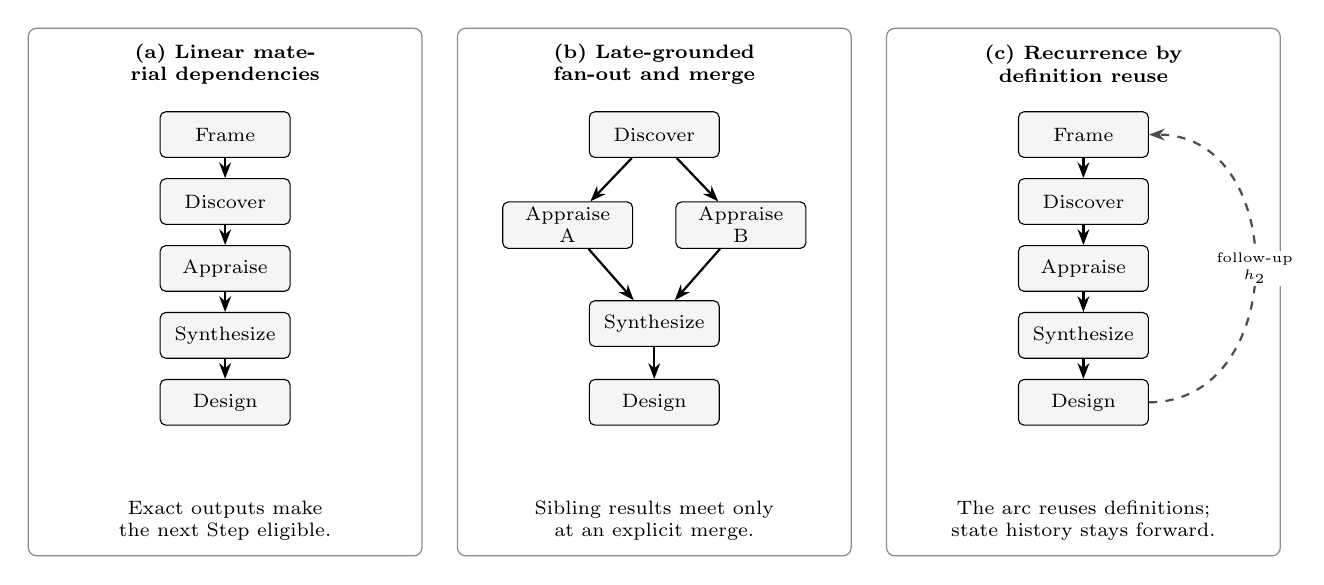
\begin{tikzpicture}[
  box/.style={draw,rounded corners=2pt,minimum width=1.65cm,minimum height=.58cm,
              align=center,font=\scriptsize,fill=black!4,inner sep=2pt},
  edge/.style={-{Stealth[length=2mm]},thick},
  reuse/.style={edge,dashed,draw=black!70},
  label/.style={font=\scriptsize,align=center},
  panel/.style={draw=black!45,rounded corners=3pt,line width=.45pt}
]
  \begin{scope}[shift={(0,0)}]
    \draw[panel] (-2.5,-.7) rectangle (2.5,6.0);
    \node[label,font=\scriptsize\bfseries,text width=4.4cm] at (0,5.55)
      {(a) Linear material dependencies};
    \node[box] (f1) at (0,4.65) {Frame};
    \node[box] (d1) at (0,3.8) {Discover};
    \node[box] (a1) at (0,2.95) {Appraise};
    \node[box] (y1) at (0,2.1) {Synthesize};
    \node[box] (z1) at (0,1.25) {Design};
    \draw[edge] (f1) -- (d1);
    \draw[edge] (d1) -- (a1);
    \draw[edge] (a1) -- (y1);
    \draw[edge] (y1) -- (z1);
    \node[label,text width=4.2cm] at (0,-.25)
      {Exact outputs make the next Step eligible.};
  \end{scope}

  \begin{scope}[xshift=5.45cm]
    \draw[panel] (-2.5,-.7) rectangle (2.5,6.0);
    \node[label,font=\scriptsize\bfseries,text width=4.4cm] at (0,5.55)
      {(b) Late-grounded fan-out and merge};
    \node[box] (d2) at (0,4.65) {Discover};
    \node[box] (a2) at (-1.1,3.5) {Appraise\\A};
    \node[box] (b2) at (1.1,3.5) {Appraise\\B};
    \node[box] (s2) at (0,2.25) {Synthesize};
    \node[box] (z2) at (0,1.25) {Design};
    \draw[edge] (d2) -- (a2);
    \draw[edge] (d2) -- (b2);
    \draw[edge] (a2) -- (s2);
    \draw[edge] (b2) -- (s2);
    \draw[edge] (s2) -- (z2);
    \node[label,text width=4.2cm] at (0,-.25)
      {Sibling results meet only at an explicit merge.};
  \end{scope}

  \begin{scope}[xshift=10.9cm]
    \draw[panel] (-2.5,-.7) rectangle (2.5,6.0);
    \node[label,font=\scriptsize\bfseries,text width=4.4cm] at (0,5.55)
      {(c) Recurrence by definition reuse};
    \node[box] (f3) at (0,4.65) {Frame};
    \node[box] (d3) at (0,3.8) {Discover};
    \node[box] (a3) at (0,2.95) {Appraise};
    \node[box] (y3) at (0,2.1) {Synthesize};
    \node[box] (z3) at (0,1.25) {Design};
    \draw[edge] (f3) -- (d3);
    \draw[edge] (d3) -- (a3);
    \draw[edge] (a3) -- (y3);
    \draw[edge] (y3) -- (z3);
    \draw[reuse]
      (z3.east) to[out=0,in=0,looseness=1.35]
      node[midway,font=\tiny,align=center,fill=white,inner sep=1pt]
        {follow-up\\$h_2$}
      (f3.east);
    \node[label,text width=4.2cm] at (0,-.25)
      {The arc reuses definitions; state history stays forward.};
  \end{scope}
\end{tikzpicture}
\caption{Three structural views of the running research-to-design Playbook.
Panel (a) shows the linear dependency chain created by exact outputs. Panel (b)
shows Discover late-grounding independent Appraise executions and Synthesize
merging their complete result set. Panel (c) adds a dashed loop arc from Design
to Frame: follow-up $h_2$ makes the same Frame definition applicable to a new
binding. The arc depicts recurrence in the Playbook definition; every accepted
execution still adds a new state along forward-only recorded history.}
\label{fig:evolution}
\end{figure*}

\subsection{A linear first reading}

At its coarsest resolution, the running Playbook forms a material-dependency chain:
Frame produces questions, Discover produces a source map, Appraise produces
evidence, Synthesize interprets the evidence, and Design applies the
interpretation. Ordering is a consequence of material availability. Synthesize
does not follow Appraise because an edge moved a token; Synthesize becomes
groundable because exact appraisal-result occurrences now fulfill its declared
input set. The next subsection refines Appraise and Synthesize into
collection-grounded fan-out and merge.

The linear reading gives two basic requirements. Intermediate writes must not
make downstream Steps applicable, because an agent can revise or abandon them.
Conversely, accepted work must have an exact identity, because a filename such
as \texttt{design.md} may be republished with identical or different bytes
during a later pass. The model therefore distinguishes an artifact
\emph{occurrence}, identified by its creating execution and state, from its
content digest.

\subsection{Dynamic branching and explicit merging}

Discover cannot know the useful fan-out before it inspects the questions and
search space. At accepted completion, Discover freezes a finite
\texttt{appraisal-requests} collection. Each member binds one Appraise
execution, so four members yield four independent executions without four
authored copies of the Step. The scheduler may run these executions
concurrently, subject to a capacity policy that does not change their logical
bindings.

A question-level Synthesize execution requires the successful results that
fulfill its exact subset of appraisal requests. The present model also requires
completion of the entire Discover expansion as a conservative readiness barrier, without
treating unrelated appraisal states as inputs or parents.
At completion, Synthesize selects a duplicate-free set of authorized states
whose result occurrences collectively cover the bound requests. The engine,
not the agent, verifies coverage and records those states as parents.

\subsection{Repetition without cyclic history}

Design emits a finite \texttt{followup-research} collection. A nonempty
collection creates a new exact binding for Frame and therefore another forward
research pass. An explicitly empty collection creates no Frame binding. Once
no other binding is eligible or running, the Playbook is \emph{quiescent}.
Quiescence means that no configured work is currently available; it is not a
proof that the design is correct, a goal has been achieved, or later human work
cannot wake the Playbook.
If every Design execution instead publishes a fresh follow-up member, forward
recurrence can continue without a fixed bound even though the recorded history
remains acyclic.

\section{Execution Model}

\subsection{Immutable task states}

Let $\mathcal{N}$ be exact artifact names, $\mathcal{O}$ immutable artifact
occurrences, and $\mathcal{W}$ material workspace checkpoints. A sealed task
state is
\begin{equation}
s=(\mathit{id}_s,w_s,A_s,C_s,Q_s,\rho_s),
\end{equation}
where $\mathit{id}_s$ is a fresh state identifier and $w_s\in\mathcal{W}$ is a
complete checkpoint. $A_s:\mathcal{N}\rightharpoonup\mathcal{O}$ is a partial
map from artifact names to visible occurrences, so a name may be absent; $C_s$
maps collection names to finite frozen member sets; $Q_s$ is a duplicate-free
set of already sealed parent-state identifiers; and $\rho_s$ records the
producing execution, definition revisions, and bound-input provenance. A state
is immutable after publication. Several states may coexist; lineage does not
mark one state as the active truth.

An occurrence identifies a publication event, not only bytes. Republishing
unchanged bytes can create a new occurrence, while an inherited artifact keeps
its prior occurrence identity. Occurrence identity lets a binding state exactly
which work it consumed without making every descendant appear fresh.

The state history $H=(S,E)$ contains edge $(p,s)$ for every $p\in Q_s$.
Because publication may name only already sealed parents and a new state
receives a fresh identity, $H$ is acyclic by construction. An ordinary
execution has one mechanically fixed parent. A merge-capable execution may
select one authorized parent when that state already covers every bound input;
selecting several distinct authorized parents creates a merge transition when
the inputs live on siblings.

\subsection{Definitions, bindings, and collections}

A Playbook revision $P^r$ is a finite set of validated Step-definition
revisions. A definition $d^r$ contains agent instructions, runtime
configuration, input declarations, readiness conditions, an output contract,
and collection relationships. Validation rejects unresolved references and
incompatible collection keys before any Session starts.

A binding $b$ contains exact ordinary occurrences and collection-member
identities. Three grounding forms are sufficient for the running example:
\begin{enumerate}
  \item an ordinary input resolves an exact named occurrence in one sealed
        state;
  \item \texttt{each}(C) enumerates one candidate grounding for every exact
        member of frozen collection $C$; and
  \item \texttt{complete-set}(R) resolves the exact successful results whose
        immutable fulfillment records cover required member set $R$.
\end{enumerate}
Collection membership is never inferred from filename patterns, directory
scans, or natural-language parsing. The producer explicitly declares a finite
collection during completion; the engine validates and freezes the declaration
inside the successor state.

Accepted publication records each declared fulfillment as an exact relation
from a result occurrence to the request member it fulfills. Failed or rejected
executions record no successful fulfillment. Claims, rather than grounding,
suppress duplicate automatic executions for already claimed exact bindings.

Readiness and input resolution are separate operations. Let $u$ be a readiness
witness set and $b$ the exact input binding. A broad condition may establish
that all Appraise requests from one Discover expansion have some successful
result, while a Synthesize binding contains only the results for one question.
The witness states in $u$ do not become input, merge candidates, or lineage
unless their occurrences also appear in $b$.

Automatic duplicate suppression uses a durable claim identity
\begin{equation}
\kappa=\operatorname{ClaimIdentity}(P^r,d^r,b,\chi),
\end{equation}
where $\chi$ is the still-open policy scope, such as ordinary-parent context or
an ancestry scope. Its canonical storage encoding is an implementation choice.
Claim acquisition and queued-execution creation form one atomic operation. A
claim names logical identity; it is not a proof of successful completion.
Explicit manual reruns receive distinct execution identities. Failure retention
and automatic retry policy remain separate decisions rather than hidden parts
of the binding.

\subsection{Executions and Sessions}

A Step execution
\begin{equation}
e=(P^r,d^r,b,A_e,K_e,o_e,W_e,\langle q_1,\ldots,q_k\rangle)
\end{equation}
binds one definition revision to one exact input, a frozen authorized candidate
set $A_e$, required coverage $K_e$, a mechanically fixed ordinary parent
$o_e$ when applicable, an isolated workspace $W_e$, and an ordered sequence of
harness Sessions. At most one Session is write-capable at a time. A continuation
Session receives the same definition, binding, and unpublished workspace; it
does not acquire another claim or create an intermediate state.

Process lifetime is therefore not the semantic boundary. A Session may exit
without completing the execution, and an execution may continue in another
Session. Conversely, a still-live process cannot mutate a state after accepted
completion. The Step execution, rather than its operating-system process, owns
the single publication decision.

\subsection{Validated atomic publication}

An agent requests completion by declaring outputs, collections, and, for a
merge, selected parent identifiers. The engine serializes completion against
continuation, suspends writes, and checks four conditions:
\begin{enumerate}
  \item every required output exists at an allowed path;
  \item every required collection is present, including an explicitly empty
        collection where emptiness is meaningful;
  \item selected parents are duplicate-free members of the candidate set frozen
        in $e$; and
  \item selected parents collectively cover every exact bound input that
        requires cross-state merge.
\end{enumerate}
After validation, the engine checkpoints the complete workspace, assigns
occurrence identities only to declared publications, freezes collections and
fulfillment relationships, constructs the state manifest, and atomically makes
the state and successful execution visible. A rejected completion publishes
nothing and leaves the execution continuable. Explicit failure closes the
execution without a successor and records failure outside the successful state
DAG.

The publication rules give the central visibility invariant:
\begin{equation}
\begin{aligned}
\operatorname{accepted}(e)
  &\Longrightarrow |\operatorname{Successors}(e)|=1,\\
\neg\operatorname{accepted}(e)
  &\Longrightarrow |\operatorname{Successors}(e)|=0.
\end{aligned}
\end{equation}
No downstream evaluation observes a partially checkpointed state or a
successful provenance record without its corresponding state.

\subsection{Reactive evaluation}

Algorithm~\ref{alg:evaluate} gives the event-driven reference behavior.
Grounding and readiness inspect a consistent snapshot of sealed history.
Exact input resolution either waits or returns $(b,A,K,o)$; the atomic
claim-and-create operation freezes those values in the execution record.
Claiming occurs before capacity-limited dispatch, so two evaluator passes cannot
create duplicate automatic executions for the same identity. A scheduler
chooses when queued work starts but cannot change what the binding means.

\begin{algorithm}[tb]
\caption{Reactive grounding, claiming, and publication}
\label{alg:evaluate}
\begin{algorithmic}[1]
\REQUIRE Playbook revision $P^r$, sealed history $H$
\STATE evaluate once when $P^r$ is attached
\LOOP
  \STATE $I \leftarrow \operatorname{Snapshot}(H)$
  \FORALL{$d^r\in P^r$}
    \FORALL{$g\in\operatorname{Ground}(d^r,I)$}
      \STATE $r\leftarrow\operatorname{ResolveExactInputs}(d^r,g,I)$
      \IF{$r=(b,A,K,o)$}
        \STATE $(ready,u)\leftarrow\operatorname{Ready}(d^r,g,b,I)$
        \IF{$ready$}
          \STATE $e\leftarrow\operatorname{ClaimAndCreate}(P^r,d^r,r)$
          \IF{$e\neq\mathsf{none}$}
            \STATE enqueue $e$
          \ENDIF
        \ENDIF
      \ENDIF
    \ENDFOR
  \ENDFOR
  \STATE dispatch queued executions within capacity
  \IF{no unclaimed binding is eligible and no work is queued or running}
    \STATE report quiescence; continue awaiting events
  \ENDIF
  \STATE $x\leftarrow\operatorname{AwaitEvent}()$
  \IF{$x=\operatorname{Completion}(e)$}
    \IF{$\operatorname{ValidateAndPublish}(e,x)$}
      \STATE add the sealed successor to $H$
    \ELSE
      \STATE keep $e$ continuable with validation errors
    \ENDIF
  \ENDIF
\ENDLOOP
\end{algorithmic}
\end{algorithm}

The loop in Algorithm~\ref{alg:evaluate} represents persistent attachment, not
busy polling. Implementations reevaluate on state-sealed and explicit manual
events, and otherwise block. A state publication may ground many executions;
capacity limits dispatch but does not defer claim identity to a mutable future
snapshot. Quiescence is reported after a complete evaluation pass finds no
eligible unclaimed grounding and no queued or running execution, regardless of
whether the preceding event published a state.

\section{The Example as a Concrete Trace}

\subsection{Linear publication boundaries}

Let the seed $S_0$ contain one initial research handoff. Frame executes in an
isolated workspace and publishes $S_1$ with a
\texttt{research-questions} occurrence. Discover binds that exact occurrence,
freezes its source decisions, and publishes $S_2$. Until each completion is
accepted, the next Step sees neither a half-written question list nor a
temporary source map.

The linear trace demonstrates why a full state, rather than an artifact bundle
alone, is the unit of publication. An agent may change code, supporting files,
and several handoffs together. A complete checkpoint makes the transition
auditable and preserves the exact material context for later inspection or a
replay attempt, while the artifact map supplies stable logical names.

\subsection{Fan-out, siblings, and coverage}

Here, $r_{iX}$ denotes the appraisal request pairing question $i$ with source
$X$, and $S_{iX}$ is the sibling state publishing the corresponding appraisal.
Suppose Discover freezes appraisal requests
$r_{1A},r_{1B},r_{2B},r_{2C}$. Four Appraise executions share parent $S_2$ but
receive distinct member bindings. Accepted results create siblings
$S_{1A},S_{1B},S_{2B},S_{2C}$ even if their wall-clock completion order differs.
The runtime never treats a later-finishing sibling as a descendant of an
earlier-finishing sibling.

Synthesize for question 1 binds only successful results fulfilling
$\{r_{1A},r_{1B}\}$. The execution's authorized candidates are frozen when the
binding is resolved. At completion, the agent may select the states that
actually supply those results; the engine accepts only a duplicate-free set
whose union covers both requests. Results for question 2 can serve as a global
readiness witness but cannot silently become parents of question 1. The same
rule lets Design merge only the exact question syntheses it uses.

Separating readiness, binding, and lineage prevents three plausible errors.
First, a state that
merely existed when a Session started does not become a parent. Second, a state
used to establish global readiness does not become an input. Third, repeating
one parent identifier does not satisfy a two-result merge. Parentage records
material dependence rather than temporal proximity.

\subsection{Another pass}

After Design publishes $S_D$, a follow-up member $h_2$ names the exact research
question that could materially change the design. The member is a new binding,
so Frame can execute again under the same definition revision. Subsequent
Discover and Appraise executions create new descendants with new occurrence
and collection identities, even if a question or source key reuses the same
human-readable text.

If Design instead freezes \texttt{followup-research} as the empty set, no Frame
execution is grounded. The Playbook becomes quiescent after all other claimed
work closes. A future manual-publication operation could add another handoff
and wake the same Playbook without rewinding or deleting earlier history; its
authority and interface remain open.

\subsection{Semantic obligations exposed by the trace}

The example yields five obligations for a compatible runtime:
\begin{enumerate}
  \item \textbf{Atomic visibility:} each accepted execution publishes one full
        state; rejected or failed work publishes none.
  \item \textbf{Topology independence:} scheduler order changes latency, not
        sibling or parent relationships.
  \item \textbf{Automatic-claim uniqueness:} each automatic claim identity
        $\kappa$ is acquired at most once.
  \item \textbf{Coverage-preserving merge:} selected parents are authorized and
        collectively supply the bound result occurrences.
  \item \textbf{Forward recurrence:} repeating a Step definition creates a new
        descendant; no concrete history edge points backward.
\end{enumerate}
Any runtime claiming compatibility with the model must preserve these
obligations. The obligations concern execution provenance and publication
topology; the semantic quality of an appraisal or design remains outside the
execution specification.

\section{Limitations and Open Decisions}

This paper specifies execution semantics and illustrates their consequences
with a constructed trace. The example demonstrates that the model represents
this research-to-design pattern; it does not establish a general expressiveness
result, scalability, liveness under failure, agent-output quality,
implementation correctness, or operational security. Claims about those
properties require separate implementation and evaluation work.

Several mechanisms remain policy rather than semantics. A production
specification must settle claim scope across sibling ancestry, retention and
retry after failure, deterministic handling of multiple valid fulfillments,
empty complete-set behavior, merge workspace conflicts, scheduler fairness,
and the representation of manual state creation. Durable publication also
requires a concrete transaction and recovery protocol that prevents a
checkpoint, manifest, claim, and database record from disagreeing after a
crash. External side effects cannot be rolled back merely because filesystem
publication fails.

The model currently assumes one authority creates automatic claims for a task.
Multiple evaluators would require fencing or a shared transactional store.
An isolated workspace is a Playbook visibility boundary, not a security
sandbox; network, subprocess, and external-tool confinement remain outside the
present semantics.
Human interaction is allowed inside a Session and through explicit manual
continuations, yet the paper does not define approval policies or how a human
selects a historical state in the interface.

Finally, the schematic notation in
Appendix~\ref{app:playbook-definition} is not a frozen serialization format.
The semantic distinctions are the intended contract: finite explicit
collections, exact bindings, atomic claims, isolated executions, validated
completion, and coverage-preserving lineage. Locking a portable syntax before
the recovery and authority decisions would turn unresolved policy into
accidental compatibility requirements.

\section{Conclusion}

Reactive Playbooks model long-running agent work as provenance-bound
transitions over immutable material states. One research-to-design definition
consequently expresses linear handoffs, runtime fan-out, concurrent siblings,
coverage-preserving merge, and later refinement without a control cursor or
cyclic history. The reference algorithm makes the governing obligations
explicit: exact grounding, atomic claiming, isolated execution, validated
single-state publication, and fail-closed parent coverage. Recovery, authority,
resource, retry, and serialization policies remain open, but implementations
can resolve those policies against the stable semantic boundary defined here.

{\small
\bibliography{references}
}

\clearpage
\appendix
\section{Schematic Playbook Definition}
\label{app:playbook-definition}

Listing~\ref{lst:playbook} records a compact definition of the running example.
The notation names the semantic relationships used in the paper without
freezing a portable serialization format. Agent instructions, harness
selection, resource policy, and output paths remain part of a complete Step
definition even where the schematic elides them.

\begin{listing}[H]
\begin{lstlisting}
playbook: research-to-design
collections:
  appraisal-requests: key(question, source)
  appraisal-results: fulfills(appraisal-requests)
  question-synthesis-requests: key(question)
  question-syntheses: fulfills(question-synthesis-requests)
  followup-research: key(handoff)
  framed-questions: fulfills(followup-research)
  design-requests: key(design)

steps:
  frame:
    input: each(followup-research)
    output: framed-questions
  discover:
    input: each(framed-questions)
    emit: [appraisal-requests,
           question-synthesis-requests,
           design-requests]
  appraise:
    input: each(appraisal-requests)
    output: appraisal-results
  synthesize:
    input: each(question-synthesis-requests)
    complete-set: required-appraisals(input)
    when: all-appraisals-from-expansion-fulfilled
    output: question-syntheses
  design:
    input: each(design-requests)
    complete-set: required-syntheses(input)
    output: [design.md, followup-research]
\end{lstlisting}
\caption{Schematic research-to-design Playbook. An initial agenda is represented
as the first member of \texttt{followup-research}; later Design executions may
emit another member or an explicitly empty collection.}
\label{lst:playbook}
\end{listing}

\clearpage
\section{Engine Design Decisions}
\label{app:engine-design-decisions}

This appendix records the engine decisions and associated authoring conventions.

\begin{enumerate}
  \item \textbf{No planning search:} the engine rolls out a fixed authored policy rather than searching for plans or inventing collaboration structures.
  \item \textbf{Fixed process, variable work:} the same Playbook can produce different numbers of executions, branches, and loop passes.
  \item \textbf{Intelligent transitions:} agents interpret evidence and choose outcomes, allowing the engine's structural rules to stay small.
  \item \textbf{No general condition language:} domain decisions live in agent instructions and artifacts rather than engine-level expressions.
  \item \textbf{Artifact-driven dependencies:} declared inputs and outputs determine readiness, independently of document order.
  \item \textbf{AND-only inputs:} every declared input is required; listing alternatives does not create an OR condition.
  \item \textbf{At least one output:} successful completion requires one valid assigned artifact, while any additional declared outputs are optional.
  \item \textbf{No engine-enforced XOR:} publishing two valid alternative outcomes is allowed; instructions must establish any required exclusivity.
  \item \textbf{Structural validation:} the engine checks publication validity, ownership, and permission without deciding whether the substantive work is good.
  \item \textbf{Atomic acceptance:} one invalid present assigned output rejects the whole completion attempt rather than accepting a partial subset.
  \item \textbf{Immutable receipts:} acceptance freezes the publication set, so repeated completion returns the same receipt and late files cannot extend it.
  \item \textbf{Ordinary mutable files:} accepted artifacts are not protected by immutable byte snapshots or an operating-system write sandbox.
  \item \textbf{Occurrence identity:} two publications count as distinct events even when their logical names and contents match.
  \item \textbf{Shared exact roles:} several steps may publish the same exact role, with each eligible occurrence enabling its own continuation.
  \item \textbf{Unique wildcard ownership:} overlapping wildcard output declarations are rejected to keep collection attribution unambiguous.
  \item \textbf{Causal input pairing:} companion artifacts must belong together through recorded provenance, not timestamps, filename order, or ``latest wins.''
  \item \textbf{Explicit ambiguity errors:} the engine rejects uncertain pairings rather than guessing, zipping alternatives, or trying every combination.
  \item \textbf{Binding-based deduplication:} observing the same ordinary input binding again does not schedule duplicate work.
  \item \textbf{Three input modes:} \texttt{single} binds one occurrence, \texttt{each} creates per-member work, and \texttt{complete} consumes a completed nonempty collection.
  \item \textbf{One collection input per step:} combining multiple collections requires explicit intermediate steps rather than implicit cross-product joins.
  \item \textbf{Batch publication:} collections become usable after accepted publication and producer shutdown, rather than streaming files into downstream work.
  \item \textbf{Accountable completeness:} queued, paused, failed, and finishing workers remain obligations instead of silently disappearing from a merge.
  \item \textbf{No implicit branch pruning:} an omitted intermediate output does not automatically discharge downstream work that was expected.
  \item \textbf{No empty consumers:} empty collections create neither item workers nor an empty \texttt{complete} execution.
  \item \textbf{Explicit no-result routing:} a disposition inside a wildcard becomes a member; one outside it can stop or route elsewhere.
  \item \textbf{Artifact-triggered recurrence:} another pass requires a fresh accepted trigger, not an overwritten file or incremented filename.
  \item \textbf{No predetermined iteration limit:} loops may continue through fresh publications, with stopping determined by the authored process.
  \item \textbf{Explicit freshness structure:} authors must put changing work inside the repeated dependency chain; parser acceptance alone does not prove freshness.
  \item \textbf{Explicit accumulated context:} agents carry useful earlier findings into new handoffs; the engine does not automatically summarize task history.
  \item \textbf{No automatic success inference:} having no eligible work does not prove that the human's objective was achieved.
  \item \textbf{Execution-scoped completion permission:} a human grant authorizes that execution and owner to finish, not particular immutable artifact contents.
  \item \textbf{Completion differs from shutdown:} downstream work waits for confirmed producer exit and output drain after acceptance.
  \item \textbf{One shared task worktree:} engine-managed coding is serialized instead of giving every execution an isolated workspace and later merging changes.
  \item \textbf{Exact coding inputs:} collection results must be consolidated before coding, although coding steps may publish collections for subsequent work.
  \item \textbf{Task-level concurrency:} the default cap is ten live sessions; excess work queues, and waiting or finishing sessions retain capacity.
  \item \textbf{No automatic retries or takeover:} recovery requires explicit ownership changes and proof that the previous owner stopped.
  \item \textbf{Manual work stays separate:} manual publications do not automatically satisfy ordinary graph dependencies or missing worker obligations.
  \item \textbf{Pinned task definitions:} library edits affect future selections rather than silently changing an existing task's Playbook.
  \item \textbf{Daemon-owned execution truth:} durable execution records drive scheduling; session metadata and UI state are repairable projections.
  \item \textbf{File-backed persistence:} the engine uses durable local records rather than adding a database or distributed execution coordinator.
  \item \textbf{Persist intent before effects:} executions and output paths are reserved before launch, while partial creation failures remain inspectable.
  \item \textbf{Names are presentation:} depth numbers and collision suffixes help people navigate artifacts but never determine provenance or scheduling.
  \item \textbf{Strict definitions:} unknown fields and unsupported syntax fail explicitly rather than acquiring guessed meanings or compatibility fallbacks.
  \item \textbf{Narrow harness support:} model selection is configurable, but current graph execution supports OMP rather than arbitrary harness integrations.
\end{enumerate}

\end{document}
